\documentclass[1p]{elsarticle_modified}
%\bibliographystyle{elsarticle-num}

%\usepackage[colorlinks]{hyperref}
%\usepackage{abbrmath_seonhwa} %\Abb, \Ascr, \Acal ,\Abf, \Afrak
\usepackage{amsfonts}
\usepackage{amssymb}
\usepackage{amsmath}
\usepackage{amsthm}
\usepackage{scalefnt}
\usepackage{amsbsy}
\usepackage{kotex}
\usepackage{caption}
\usepackage{subfig}
\usepackage{color}
\usepackage{graphicx}
\usepackage{xcolor} %% white, black, red, green, blue, cyan, magenta, yellow
\usepackage{float}
\usepackage{setspace}
\usepackage{hyperref}

\usepackage{tikz}
\usetikzlibrary{arrows}

\usepackage{multirow}
\usepackage{array} % fixed length table
\usepackage{hhline}

%%%%%%%%%%%%%%%%%%%%%
\makeatletter
\renewcommand*\env@matrix[1][\arraystretch]{%
	\edef\arraystretch{#1}%
	\hskip -\arraycolsep
	\let\@ifnextchar\new@ifnextchar
	\array{*\c@MaxMatrixCols c}}
\makeatother %https://tex.stackexchange.com/questions/14071/how-can-i-increase-the-line-spacing-in-a-matrix
%%%%%%%%%%%%%%%

\usepackage[normalem]{ulem}

\newcommand{\msout}[1]{\ifmmode\text{\sout{\ensuremath{#1}}}\else\sout{#1}\fi}
%SOURCE: \msout is \stkout macro in https://tex.stackexchange.com/questions/20609/strikeout-in-math-mode

\newcommand{\cancel}[1]{
	\ifmmode
	{\color{red}\msout{#1}}
	\else
	{\color{red}\sout{#1}}
	\fi
}

\newcommand{\add}[1]{
	{\color{blue}\uwave{#1}}
}

\newcommand{\replace}[2]{
	\ifmmode
	{\color{red}\msout{#1}}{\color{blue}\uwave{#2}}
	\else
	{\color{red}\sout{#1}}{\color{blue}\uwave{#2}}
	\fi
}

\newcommand{\Sol}{\mathcal{S}} %segment
\newcommand{\D}{D} %diagram
\newcommand{\A}{\mathcal{A}} %arc


%%%%%%%%%%%%%%%%%%%%%%%%%%%%%5 test

\def\sl{\operatorname{\textup{SL}}(2,\Cbb)}
\def\psl{\operatorname{\textup{PSL}}(2,\Cbb)}
\def\quan{\mkern 1mu \triangleright \mkern 1mu}

\theoremstyle{definition}
\newtheorem{thm}{Theorem}[section]
\newtheorem{prop}[thm]{Proposition}
\newtheorem{lem}[thm]{Lemma}
\newtheorem{ques}[thm]{Question}
\newtheorem{cor}[thm]{Corollary}
\newtheorem{defn}[thm]{Definition}
\newtheorem{exam}[thm]{Example}
\newtheorem{rmk}[thm]{Remark}
\newtheorem{alg}[thm]{Algorithm}

\newcommand{\I}{\sqrt{-1}}
\begin{document}

%\begin{frontmatter}
%
%\title{Boundary parabolic representations of knots up to 8 crossings}
%
%%% Group authors per affiliation:
%\author{Yunhi Cho} 
%\address{Department of Mathematics, University of Seoul, Seoul, Korea}
%\ead{yhcho@uos.ac.kr}
%
%
%\author{Seonhwa Kim} %\fnref{s_kim}}
%\address{Center for Geometry and Physics, Institute for Basic Science, Pohang, 37673, Korea}
%\ead{ryeona17@ibs.re.kr}
%
%\author{Hyuk Kim}
%\address{Department of Mathematical Sciences, Seoul National University, Seoul 08826, Korea}
%\ead{hyukkim@snu.ac.kr}
%
%\author{Seokbeom Yoon}
%\address{Department of Mathematical Sciences, Seoul National University, Seoul, 08826,  Korea}
%\ead{sbyoon15@snu.ac.kr}
%
%\begin{abstract}
%We find all boundary parabolic representation of knots up to 8 crossings.
%
%\end{abstract}
%\begin{keyword}
%    \MSC[2010] 57M25 
%\end{keyword}
%
%\end{frontmatter}

%\linenumbers
%\tableofcontents
%
\newcommand\colored[1]{\textcolor{white}{\rule[-0.35ex]{0.8em}{1.4ex}}\kern-0.8em\color{red} #1}%
%\newcommand\colored[1]{\textcolor{white}{ #1}\kern-2.17ex	\textcolor{white}{ #1}\kern-1.81ex	\textcolor{white}{ #1}\kern-2.15ex\color{red}#1	}

{\Large $\underline{12a_{0684}~(K12a_{0684})}$}

\setlength{\tabcolsep}{10pt}
\renewcommand{\arraystretch}{1.6}
\vspace{1cm}\begin{tabular}{m{100pt}>{\centering\arraybackslash}m{274pt}}
\multirow{5}{120pt}{
	\centering
	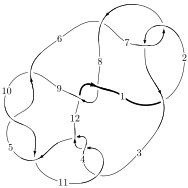
\includegraphics[width=112pt]{../../../GIT/diagram.site/Diagrams/png/1485_12a_0684.png}\\
\ \ \ A knot diagram\footnotemark}&
\allowdisplaybreaks
\textbf{Linearized knot diagam} \\
\cline{2-2}
 &
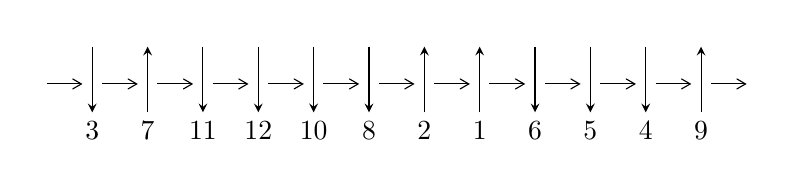
\begin{tikzpicture}[x=20pt, y=17pt]
	% nodes
	\node (C0) at (0, 0) {};
	\node (C1) at (1, 0) {};
	\node (C1U) at (1, +1) {};
	\node (C1D) at (1, -1) {3};

	\node (C2) at (2, 0) {};
	\node (C2U) at (2, +1) {};
	\node (C2D) at (2, -1) {7};

	\node (C3) at (3, 0) {};
	\node (C3U) at (3, +1) {};
	\node (C3D) at (3, -1) {11};

	\node (C4) at (4, 0) {};
	\node (C4U) at (4, +1) {};
	\node (C4D) at (4, -1) {12};

	\node (C5) at (5, 0) {};
	\node (C5U) at (5, +1) {};
	\node (C5D) at (5, -1) {10};

	\node (C6) at (6, 0) {};
	\node (C6U) at (6, +1) {};
	\node (C6D) at (6, -1) {8};

	\node (C7) at (7, 0) {};
	\node (C7U) at (7, +1) {};
	\node (C7D) at (7, -1) {2};

	\node (C8) at (8, 0) {};
	\node (C8U) at (8, +1) {};
	\node (C8D) at (8, -1) {1};

	\node (C9) at (9, 0) {};
	\node (C9U) at (9, +1) {};
	\node (C9D) at (9, -1) {6};

	\node (C10) at (10, 0) {};
	\node (C10U) at (10, +1) {};
	\node (C10D) at (10, -1) {5};

	\node (C11) at (11, 0) {};
	\node (C11U) at (11, +1) {};
	\node (C11D) at (11, -1) {4};

	\node (C12) at (12, 0) {};
	\node (C12U) at (12, +1) {};
	\node (C12D) at (12, -1) {9};
	\node (C13) at (13, 0) {};

	% arrows
	\draw[->,>={angle 60}]
	(C0) edge (C1) (C1) edge (C2) (C2) edge (C3) (C3) edge (C4) (C4) edge (C5) (C5) edge (C6) (C6) edge (C7) (C7) edge (C8) (C8) edge (C9) (C9) edge (C10) (C10) edge (C11) (C11) edge (C12) (C12) edge (C13) ;	\draw[->,>=stealth]
	(C1U) edge (C1D) (C2D) edge (C2U) (C3U) edge (C3D) (C4U) edge (C4D) (C5U) edge (C5D) (C6U) edge (C6D) (C7D) edge (C7U) (C8D) edge (C8U) (C9U) edge (C9D) (C10U) edge (C10D) (C11U) edge (C11D) (C12D) edge (C12U) ;
	\end{tikzpicture} \\
\hhline{~~} \\& 
\textbf{Solving Sequence} \\ \cline{2-2} 
 &
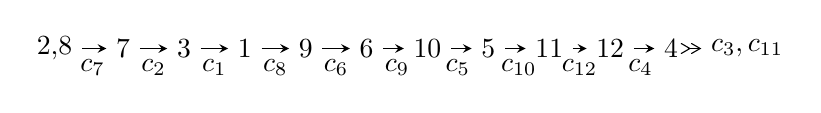
\begin{tikzpicture}[x=22pt, y=7pt]
	% node
	\node (A0) at (-1/8, 0) {2,8};
	\node (A1) at (1, 0) {7};
	\node (A2) at (2, 0) {3};
	\node (A3) at (3, 0) {1};
	\node (A4) at (4, 0) {9};
	\node (A5) at (5, 0) {6};
	\node (A6) at (6, 0) {10};
	\node (A7) at (7, 0) {5};
	\node (A8) at (8, 0) {11};
	\node (A9) at (9, 0) {12};
	\node (A10) at (10, 0) {4};
	\node (C1) at (1/2, -1) {$c_{7}$};
	\node (C2) at (3/2, -1) {$c_{2}$};
	\node (C3) at (5/2, -1) {$c_{1}$};
	\node (C4) at (7/2, -1) {$c_{8}$};
	\node (C5) at (9/2, -1) {$c_{6}$};
	\node (C6) at (11/2, -1) {$c_{9}$};
	\node (C7) at (13/2, -1) {$c_{5}$};
	\node (C8) at (15/2, -1) {$c_{10}$};
	\node (C9) at (17/2, -1) {$c_{12}$};
	\node (C10) at (19/2, -1) {$c_{4}$};
	\node (A11) at (45/4, 0) {$c_{3},c_{11}$};

	% edge
	\draw[->,>=stealth]	
	(A0) edge (A1) (A1) edge (A2) (A2) edge (A3) (A3) edge (A4) (A4) edge (A5) (A5) edge (A6) (A6) edge (A7) (A7) edge (A8) (A8) edge (A9) (A9) edge (A10) ;
	\draw[->>,>={angle 60}]	
	(A10) edge (A11);
\end{tikzpicture} \\ 

\end{tabular} \\

\footnotetext{
The image of knot diagram is generated by the software ``\textbf{Draw programme}" developed by Andrew Bartholomew(\url{http://www.layer8.co.uk/maths/draw/index.htm\#Running-draw}), where we modified some parts for our purpose(\url{https://github.com/CATsTAILs/LinksPainter}).
}\phantom \\ \newline 
\centering \textbf{Ideals for irreducible components\footnotemark of $X_{\text{par}}$} 
 
\begin{align*}
I^u_{1}&=\langle 
u^{67}+u^{66}+\cdots+3 u^2+1\rangle \\
\\
\end{align*}
\raggedright * 1 irreducible components of $\dim_{\mathbb{C}}=0$, with total 67 representations.\\
\footnotetext{All coefficients of polynomials are rational numbers. But the coefficients are sometimes approximated in decimal forms when there is not enough margin.}
\newpage
\renewcommand{\arraystretch}{1}
\centering \section*{I. $I^u_{1}= \langle u^{67}+u^{66}+\cdots+3 u^2+1 \rangle$}
\flushleft \textbf{(i) Arc colorings}\\
\begin{tabular}{m{7pt} m{180pt} m{7pt} m{180pt} }
\flushright $a_{2}=$&$\begin{pmatrix}0\\u\end{pmatrix}$ \\
\flushright $a_{8}=$&$\begin{pmatrix}1\\0\end{pmatrix}$ \\
\flushright $a_{7}=$&$\begin{pmatrix}1\\u^2\end{pmatrix}$ \\
\flushright $a_{3}=$&$\begin{pmatrix}u\\u^3+u\end{pmatrix}$ \\
\flushright $a_{1}=$&$\begin{pmatrix}u^3\\u^5+u^3+u\end{pmatrix}$ \\
\flushright $a_{9}=$&$\begin{pmatrix}- u^8- u^6- u^4+1\\- u^{10}-2 u^8-3 u^6-2 u^4- u^2\end{pmatrix}$ \\
\flushright $a_{6}=$&$\begin{pmatrix}u^2+1\\u^2\end{pmatrix}$ \\
\flushright $a_{10}=$&$\begin{pmatrix}u^{14}+3 u^{12}+6 u^{10}+7 u^8+6 u^6+4 u^4+2 u^2+1\\u^{14}+2 u^{12}+3 u^{10}+2 u^8- u^2\end{pmatrix}$ \\
\flushright $a_{5}=$&$\begin{pmatrix}u^{26}+5 u^{24}+\cdots+3 u^2+1\\u^{26}+4 u^{24}+\cdots-2 u^4+u^2\end{pmatrix}$ \\
\flushright $a_{11}=$&$\begin{pmatrix}u^{38}+7 u^{36}+\cdots+4 u^2+1\\u^{38}+6 u^{36}+\cdots+2 u^4- u^2\end{pmatrix}$ \\
\flushright $a_{12}=$&$\begin{pmatrix}u^{13}+2 u^{11}+3 u^9+2 u^7- u\\u^{15}+3 u^{13}+6 u^{11}+7 u^9+6 u^7+4 u^5+2 u^3+u\end{pmatrix}$ \\
\flushright $a_{4}=$&$\begin{pmatrix}- u^{54}-9 u^{52}+\cdots+4 u^2+1\\- u^{56}-10 u^{54}+\cdots-34 u^6-10 u^4\end{pmatrix}$\\&\end{tabular}
\flushleft \textbf{(ii) Obstruction class $= -1$}\\~\\
\flushleft \textbf{(iii) Cusp Shapes $= -4 u^{65}-4 u^{64}+\cdots-16 u-6$}\\~\\
\newpage\renewcommand{\arraystretch}{1}
\flushleft \textbf{(iv) u-Polynomials at the component}\newline \\
\begin{tabular}{m{50pt}|m{274pt}}
Crossings & \hspace{64pt}u-Polynomials at each crossing \\
\hline $$\begin{aligned}c_{1},c_{6}\end{aligned}$$&$\begin{aligned}
&u^{67}+23 u^{66}+\cdots-6 u-1
\end{aligned}$\\
\hline $$\begin{aligned}c_{2},c_{7}\end{aligned}$$&$\begin{aligned}
&u^{67}+u^{66}+\cdots+3 u^2+1
\end{aligned}$\\
\hline $$\begin{aligned}c_{3},c_{4},c_{11}\end{aligned}$$&$\begin{aligned}
&u^{67}+u^{66}+\cdots+2 u+1
\end{aligned}$\\
\hline $$\begin{aligned}c_{5},c_{9},c_{10}\end{aligned}$$&$\begin{aligned}
&u^{67}-3 u^{66}+\cdots+11 u-16
\end{aligned}$\\
\hline $$\begin{aligned}c_{8},c_{12}\end{aligned}$$&$\begin{aligned}
&u^{67}-5 u^{66}+\cdots-32 u+16
\end{aligned}$\\
\hline
\end{tabular}\\~\\
\newpage\renewcommand{\arraystretch}{1}
\flushleft \textbf{(v) Riley Polynomials at the component}\newline \\
\begin{tabular}{m{50pt}|m{274pt}}
Crossings & \hspace{64pt}Riley Polynomials at each crossing \\
\hline $$\begin{aligned}c_{1},c_{6}\end{aligned}$$&$\begin{aligned}
&y^{67}+43 y^{66}+\cdots-14 y-1
\end{aligned}$\\
\hline $$\begin{aligned}c_{2},c_{7}\end{aligned}$$&$\begin{aligned}
&y^{67}+23 y^{66}+\cdots-6 y-1
\end{aligned}$\\
\hline $$\begin{aligned}c_{3},c_{4},c_{11}\end{aligned}$$&$\begin{aligned}
&y^{67}-53 y^{66}+\cdots-6 y-1
\end{aligned}$\\
\hline $$\begin{aligned}c_{5},c_{9},c_{10}\end{aligned}$$&$\begin{aligned}
&y^{67}+63 y^{66}+\cdots-1383 y-256
\end{aligned}$\\
\hline $$\begin{aligned}c_{8},c_{12}\end{aligned}$$&$\begin{aligned}
&y^{67}+35 y^{66}+\cdots-12512 y-256
\end{aligned}$\\
\hline
\end{tabular}\\~\\
\newpage\flushleft \textbf{(vi) Complex Volumes and Cusp Shapes}
$$\begin{array}{c|c|c}  
\text{Solutions to }I^u_{1}& \I (\text{vol} + \sqrt{-1}CS) & \text{Cusp shape}\\
 \hline 
\begin{aligned}
u &= -0.803360 + 0.638492 I\end{aligned}
 & \phantom{-}2.78379 + 9.20045 I & -4.00000 - 5.04305 I \\ \hline\begin{aligned}
u &= -0.803360 - 0.638492 I\end{aligned}
 & \phantom{-}2.78379 - 9.20045 I & -4.00000 + 5.04305 I \\ \hline\begin{aligned}
u &= \phantom{-}0.800124 + 0.647068 I\end{aligned}
 & \phantom{-}7.09459 - 4.72698 I & \phantom{-0.000000 -}0. + 2.48714 I \\ \hline\begin{aligned}
u &= \phantom{-}0.800124 - 0.647068 I\end{aligned}
 & \phantom{-}7.09459 + 4.72698 I & \phantom{-0.000000 } 0. - 2.48714 I \\ \hline\begin{aligned}
u &= -0.794421 + 0.657199 I\end{aligned}
 & \phantom{-}3.54889 + 0.19967 I & \phantom{-0.000000 } 0 \\ \hline\begin{aligned}
u &= -0.794421 - 0.657199 I\end{aligned}
 & \phantom{-}3.54889 - 0.19967 I & \phantom{-0.000000 } 0 \\ \hline\begin{aligned}
u &= -0.729773 + 0.636528 I\end{aligned}
 & \phantom{-}0.83498 + 2.07700 I & -1.30731 - 4.65040 I \\ \hline\begin{aligned}
u &= -0.729773 - 0.636528 I\end{aligned}
 & \phantom{-}0.83498 - 2.07700 I & -1.30731 + 4.65040 I \\ \hline\begin{aligned}
u &= \phantom{-}0.701441 + 0.764368 I\end{aligned}
 & \phantom{-}0.332471 - 0.137935 I & -4.00000 + 0. I\phantom{ +0.000000I} \\ \hline\begin{aligned}
u &= \phantom{-}0.701441 - 0.764368 I\end{aligned}
 & \phantom{-}0.332471 + 0.137935 I & -4.00000 + 0. I\phantom{ +0.000000I} \\ \hline\begin{aligned}
u &= \phantom{-}0.751806 + 0.599939 I\end{aligned}
 & -4.30064 - 4.22428 I & -7.11593 + 3.82963 I \\ \hline\begin{aligned}
u &= \phantom{-}0.751806 - 0.599939 I\end{aligned}
 & -4.30064 + 4.22428 I & -7.11593 - 3.82963 I \\ \hline\begin{aligned}
u &= \phantom{-}0.022057 + 1.053290 I\end{aligned}
 & -4.58704 + 1.51218 I & -9.45944 - 4.55261 I \\ \hline\begin{aligned}
u &= \phantom{-}0.022057 - 1.053290 I\end{aligned}
 & -4.58704 - 1.51218 I & -9.45944 + 4.55261 I \\ \hline\begin{aligned}
u &= \phantom{-}0.096493 + 1.057100 I\end{aligned}
 & -2.57943 - 0.08281 I & -8.50549 + 0. I\phantom{ +0.000000I} \\ \hline\begin{aligned}
u &= \phantom{-}0.096493 - 1.057100 I\end{aligned}
 & -2.57943 + 0.08281 I & -8.50549 + 0. I\phantom{ +0.000000I} \\ \hline\begin{aligned}
u &= -0.669102 + 0.844952 I\end{aligned}
 & \phantom{-}3.28932 - 2.58275 I & \phantom{-0.000000 } 0 \\ \hline\begin{aligned}
u &= -0.669102 - 0.844952 I\end{aligned}
 & \phantom{-}3.28932 + 2.58275 I & \phantom{-0.000000 } 0 \\ \hline\begin{aligned}
u &= \phantom{-}0.529127 + 0.939240 I\end{aligned}
 & -0.06741 + 5.98627 I & \phantom{-0.000000 } 0 \\ \hline\begin{aligned}
u &= \phantom{-}0.529127 - 0.939240 I\end{aligned}
 & -0.06741 - 5.98627 I & \phantom{-0.000000 } 0 \\ \hline\begin{aligned}
u &= \phantom{-}0.647786 + 0.655651 I\end{aligned}
 & \phantom{-}0.241433 + 0.748431 I & -4.13794 - 3.90803 I \\ \hline\begin{aligned}
u &= \phantom{-}0.647786 - 0.655651 I\end{aligned}
 & \phantom{-}0.241433 - 0.748431 I & -4.13794 + 3.90803 I \\ \hline\begin{aligned}
u &= -0.092376 + 1.074670 I\end{aligned}
 & \phantom{-}0.91363 - 4.29574 I & \phantom{-0.000000 } 0 \\ \hline\begin{aligned}
u &= -0.092376 - 1.074670 I\end{aligned}
 & \phantom{-}0.91363 + 4.29574 I & \phantom{-0.000000 } 0 \\ \hline\begin{aligned}
u &= -0.028914 + 1.086230 I\end{aligned}
 & -9.95694 - 3.35433 I & -14.2561 + 0. I\phantom{ +0.000000I} \\ \hline\begin{aligned}
u &= -0.028914 - 1.086230 I\end{aligned}
 & -9.95694 + 3.35433 I & -14.2561 + 0. I\phantom{ +0.000000I} \\ \hline\begin{aligned}
u &= \phantom{-}0.087961 + 1.086010 I\end{aligned}
 & -3.41796 + 8.65689 I & \phantom{-0.000000 } 0 \\ \hline\begin{aligned}
u &= \phantom{-}0.087961 - 1.086010 I\end{aligned}
 & -3.41796 - 8.65689 I & \phantom{-0.000000 } 0 \\ \hline\begin{aligned}
u &= -0.558836 + 0.972282 I\end{aligned}
 & \phantom{-}3.64416 - 1.88415 I & \phantom{-0.000000 } 0 \\ \hline\begin{aligned}
u &= -0.558836 - 0.972282 I\end{aligned}
 & \phantom{-}3.64416 + 1.88415 I & \phantom{-0.000000 } 0\\
 \hline 
 \end{array}$$\newpage$$\begin{array}{c|c|c}  
\text{Solutions to }I^u_{1}& \I (\text{vol} + \sqrt{-1}CS) & \text{Cusp shape}\\
 \hline 
\begin{aligned}
u &= \phantom{-}0.567085 + 0.994839 I\end{aligned}
 & -0.56916 - 2.29584 I & \phantom{-0.000000 } 0 \\ \hline\begin{aligned}
u &= \phantom{-}0.567085 - 0.994839 I\end{aligned}
 & -0.56916 + 2.29584 I & \phantom{-0.000000 } 0 \\ \hline\begin{aligned}
u &= \phantom{-}0.672545 + 0.927735 I\end{aligned}
 & -0.16758 + 5.42739 I & \phantom{-0.000000 } 0 \\ \hline\begin{aligned}
u &= \phantom{-}0.672545 - 0.927735 I\end{aligned}
 & -0.16758 - 5.42739 I & \phantom{-0.000000 } 0 \\ \hline\begin{aligned}
u &= -0.762268 + 0.857726 I\end{aligned}
 & \phantom{-}6.75974 + 1.69859 I & \phantom{-0.000000 } 0 \\ \hline\begin{aligned}
u &= -0.762268 - 0.857726 I\end{aligned}
 & \phantom{-}6.75974 - 1.69859 I & \phantom{-0.000000 } 0 \\ \hline\begin{aligned}
u &= \phantom{-}0.760734 + 0.867270 I\end{aligned}
 & \phantom{-}10.68380 + 2.86836 I & \phantom{-0.000000 } 0 \\ \hline\begin{aligned}
u &= \phantom{-}0.760734 - 0.867270 I\end{aligned}
 & \phantom{-}10.68380 - 2.86836 I & \phantom{-0.000000 } 0 \\ \hline\begin{aligned}
u &= -0.757930 + 0.876228 I\end{aligned}
 & \phantom{-}6.70343 - 7.43134 I & \phantom{-0.000000 } 0 \\ \hline\begin{aligned}
u &= -0.757930 - 0.876228 I\end{aligned}
 & \phantom{-}6.70343 + 7.43134 I & \phantom{-0.000000 } 0 \\ \hline\begin{aligned}
u &= -0.650192 + 0.524941 I\end{aligned}
 & -4.92057 - 2.05889 I & -8.44124 + 3.45168 I \\ \hline\begin{aligned}
u &= -0.650192 - 0.524941 I\end{aligned}
 & -4.92057 + 2.05889 I & -8.44124 - 3.45168 I \\ \hline\begin{aligned}
u &= -0.271313 + 0.769915 I\end{aligned}
 & -4.53163 - 2.07205 I & -11.22172 + 5.13585 I \\ \hline\begin{aligned}
u &= -0.271313 - 0.769915 I\end{aligned}
 & -4.53163 + 2.07205 I & -11.22172 - 5.13585 I \\ \hline\begin{aligned}
u &= \phantom{-}0.649976 + 0.994312 I\end{aligned}
 & -0.77232 + 4.37126 I & \phantom{-0.000000 } 0 \\ \hline\begin{aligned}
u &= \phantom{-}0.649976 - 0.994312 I\end{aligned}
 & -0.77232 - 4.37126 I & \phantom{-0.000000 } 0 \\ \hline\begin{aligned}
u &= -0.631035 + 1.015860 I\end{aligned}
 & -6.25413 - 2.96400 I & \phantom{-0.000000 } 0 \\ \hline\begin{aligned}
u &= -0.631035 - 1.015860 I\end{aligned}
 & -6.25413 + 2.96400 I & \phantom{-0.000000 } 0 \\ \hline\begin{aligned}
u &= -0.671448 + 1.010100 I\end{aligned}
 & -0.27092 - 7.45199 I & \phantom{-0.000000 } 0 \\ \hline\begin{aligned}
u &= -0.671448 - 1.010100 I\end{aligned}
 & -0.27092 + 7.45199 I & \phantom{-0.000000 } 0 \\ \hline\begin{aligned}
u &= \phantom{-}0.669526 + 1.027320 I\end{aligned}
 & -5.55831 + 9.64000 I & \phantom{-0.000000 } 0 \\ \hline\begin{aligned}
u &= \phantom{-}0.669526 - 1.027320 I\end{aligned}
 & -5.55831 - 9.64000 I & \phantom{-0.000000 } 0 \\ \hline\begin{aligned}
u &= -0.701809 + 1.019670 I\end{aligned}
 & \phantom{-}2.45618 - 5.84517 I & \phantom{-0.000000 } 0 \\ \hline\begin{aligned}
u &= -0.701809 - 1.019670 I\end{aligned}
 & \phantom{-}2.45618 + 5.84517 I & \phantom{-0.000000 } 0 \\ \hline\begin{aligned}
u &= \phantom{-}0.701023 + 1.026000 I\end{aligned}
 & \phantom{-}5.95293 + 10.38420 I & \phantom{-0.000000 } 0 \\ \hline\begin{aligned}
u &= \phantom{-}0.701023 - 1.026000 I\end{aligned}
 & \phantom{-}5.95293 - 10.38420 I & \phantom{-0.000000 } 0 \\ \hline\begin{aligned}
u &= -0.699473 + 1.030620 I\end{aligned}
 & \phantom{-}1.6032 - 14.8599 I & \phantom{-0.000000 } 0 \\ \hline\begin{aligned}
u &= -0.699473 - 1.030620 I\end{aligned}
 & \phantom{-}1.6032 + 14.8599 I & \phantom{-0.000000 } 0 \\ \hline\begin{aligned}
u &= \phantom{-}0.634928 + 0.324518 I\end{aligned}
 & \phantom{-}1.12766 + 6.71660 I & -2.59886 - 5.83457 I \\ \hline\begin{aligned}
u &= \phantom{-}0.634928 - 0.324518 I\end{aligned}
 & \phantom{-}1.12766 - 6.71660 I & -2.59886 + 5.83457 I\\
 \hline 
 \end{array}$$\newpage$$\begin{array}{c|c|c}  
\text{Solutions to }I^u_{1}& \I (\text{vol} + \sqrt{-1}CS) & \text{Cusp shape}\\
 \hline 
\begin{aligned}
u &= -0.616892 + 0.299152 I\end{aligned}
 & \phantom{-}5.31573 - 2.35989 I & \phantom{-}1.86076 + 3.06293 I \\ \hline\begin{aligned}
u &= -0.616892 - 0.299152 I\end{aligned}
 & \phantom{-}5.31573 + 2.35989 I & \phantom{-}1.86076 - 3.06293 I \\ \hline\begin{aligned}
u &= \phantom{-}0.597047 + 0.266295 I\end{aligned}
 & \phantom{-}1.62809 - 2.00771 I & -1.45361 + 0.46558 I \\ \hline\begin{aligned}
u &= \phantom{-}0.597047 - 0.266295 I\end{aligned}
 & \phantom{-}1.62809 + 2.00771 I & -1.45361 - 0.46558 I \\ \hline\begin{aligned}
u &= \phantom{-}0.255920 + 0.412745 I\end{aligned}
 & -0.118014 + 0.819285 I & -3.06015 - 8.28989 I \\ \hline\begin{aligned}
u &= \phantom{-}0.255920 - 0.412745 I\end{aligned}
 & -0.118014 - 0.819285 I & -3.06015 + 8.28989 I \\ \hline\begin{aligned}
u &= -0.412874\phantom{ +0.000000I}\end{aligned}
 & -2.43012\phantom{ +0.000000I} & -1.69860\phantom{ +0.000000I}\\
 \hline 
 \end{array}$$\newpage
\newpage\renewcommand{\arraystretch}{1}
\centering \section*{ II. u-Polynomials}
\begin{tabular}{m{50pt}|m{274pt}}
Crossings & \hspace{64pt}u-Polynomials at each crossing \\
\hline $$\begin{aligned}c_{1},c_{6}\end{aligned}$$&$\begin{aligned}
&u^{67}+23 u^{66}+\cdots-6 u-1
\end{aligned}$\\
\hline $$\begin{aligned}c_{2},c_{7}\end{aligned}$$&$\begin{aligned}
&u^{67}+u^{66}+\cdots+3 u^2+1
\end{aligned}$\\
\hline $$\begin{aligned}c_{3},c_{4},c_{11}\end{aligned}$$&$\begin{aligned}
&u^{67}+u^{66}+\cdots+2 u+1
\end{aligned}$\\
\hline $$\begin{aligned}c_{5},c_{9},c_{10}\end{aligned}$$&$\begin{aligned}
&u^{67}-3 u^{66}+\cdots+11 u-16
\end{aligned}$\\
\hline $$\begin{aligned}c_{8},c_{12}\end{aligned}$$&$\begin{aligned}
&u^{67}-5 u^{66}+\cdots-32 u+16
\end{aligned}$\\
\hline
\end{tabular}\newpage\renewcommand{\arraystretch}{1}
\centering \section*{ III. Riley Polynomials}
\begin{tabular}{m{50pt}|m{274pt}}
Crossings & \hspace{64pt}Riley Polynomials at each crossing \\
\hline $$\begin{aligned}c_{1},c_{6}\end{aligned}$$&$\begin{aligned}
&y^{67}+43 y^{66}+\cdots-14 y-1
\end{aligned}$\\
\hline $$\begin{aligned}c_{2},c_{7}\end{aligned}$$&$\begin{aligned}
&y^{67}+23 y^{66}+\cdots-6 y-1
\end{aligned}$\\
\hline $$\begin{aligned}c_{3},c_{4},c_{11}\end{aligned}$$&$\begin{aligned}
&y^{67}-53 y^{66}+\cdots-6 y-1
\end{aligned}$\\
\hline $$\begin{aligned}c_{5},c_{9},c_{10}\end{aligned}$$&$\begin{aligned}
&y^{67}+63 y^{66}+\cdots-1383 y-256
\end{aligned}$\\
\hline $$\begin{aligned}c_{8},c_{12}\end{aligned}$$&$\begin{aligned}
&y^{67}+35 y^{66}+\cdots-12512 y-256
\end{aligned}$\\
\hline
\end{tabular}
\vskip 2pc
\end{document}